\chapter*{Anexo A --- Diagramas de Atividades}
\label{anexo}
%\addtocontents{toc}{\protect\contentsline {chapter}{Anexo A --- Diagramas de Atividades}{58}}
Neste anexo s�o apresentados os diagramas de atividades UML modelados para a implementa��o do sistema. S�o apresentados os diagrama de atividade detalhando, assim, cada caso de uso do sistema.
\begin{figure}[!h]
\centering
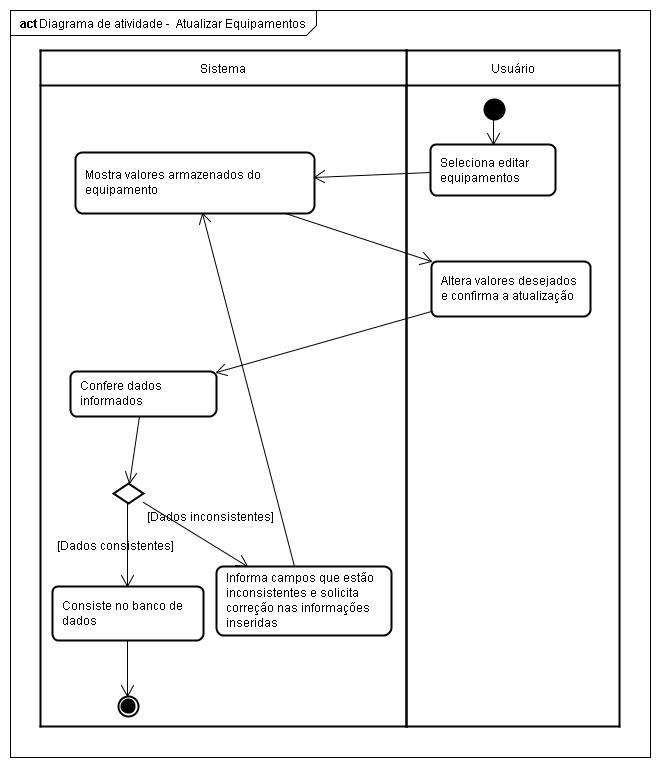
\includegraphics[width=14cm, height=15cm]{imagens-tc2/atividades/atualizarequipamentos.jpg}
%\caption{Diagrama de atividade - Atualizar Equipamentos}
\label{fig:Diagrama de atividade - Atualizar Equipamentos}
\end{figure}
\begin{figure}
\centering
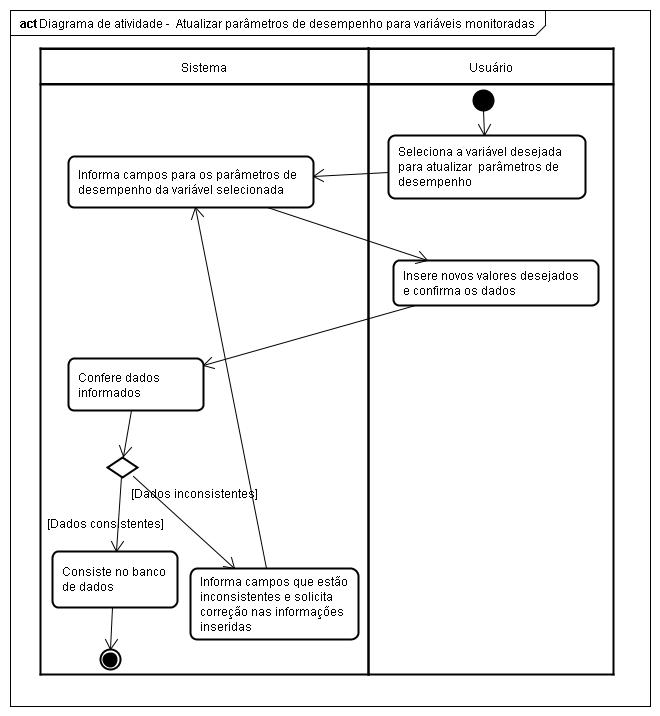
\includegraphics[width=15cm, height=20cm]{imagens-tc2/atividades/atualizarparametros.jpg}
%\caption{Diagrama de atividade - Atualizar par�metros de desempenho para vari�veis monitoradas}
\label{fig:Diagrama de atividade - Atualizar par�metros de desempenho para vari�veis monitoradas}
\end{figure}
\begin{figure}
\centering
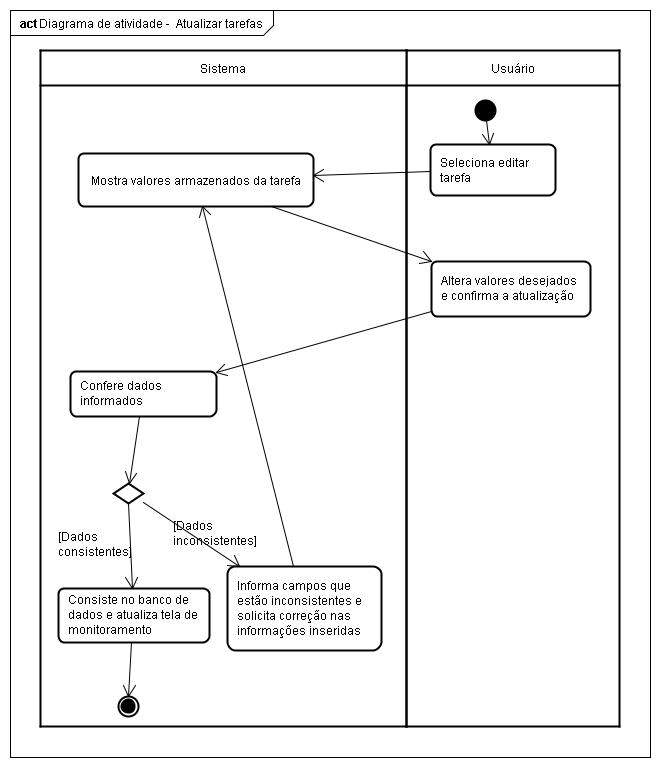
\includegraphics[width=15cm, height=20cm]{imagens-tc2/atividades/atualizartarefas.jpg}
%\caption{Diagrama de atividade - Atualizar tarefas}
\label{fig:Diagrama de atividade - Atualizar tarefas}
\end{figure}
\begin{figure}
\centering
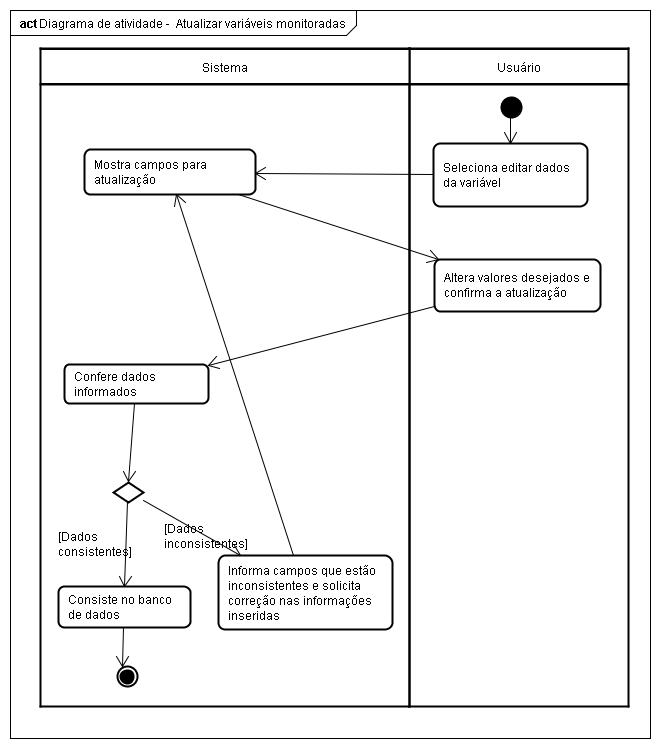
\includegraphics[width=15cm, height=20cm]{imagens-tc2/atividades/atualizarvariaveis.jpg}
%\caption{Diagrama de atividade - Atualizar vari�veis monitoradas}
\label{fig:Diagrama de atividade - Atualizar vari�veis monitoradas}
\end{figure}
\begin{figure}
\centering
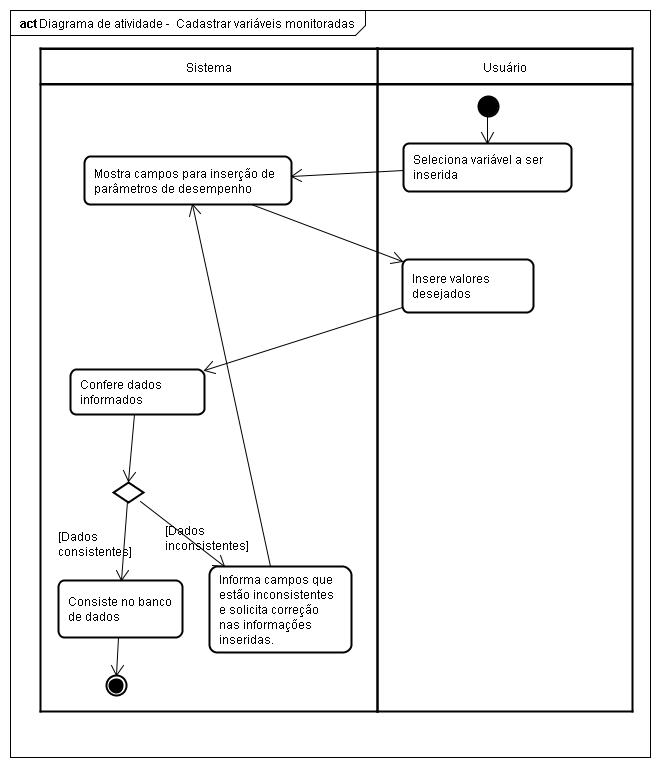
\includegraphics[width=15cm, height=20cm]{imagens-tc2/atividades/cadastrarvariaveis.jpg}
%\caption{Diagrama de atividade - Cadastrar vari�veis monitoradas}
\label{fig:Diagrama de atividade - Cadastrar vari�veis monitoradas}
\end{figure}
\begin{figure}
\centering
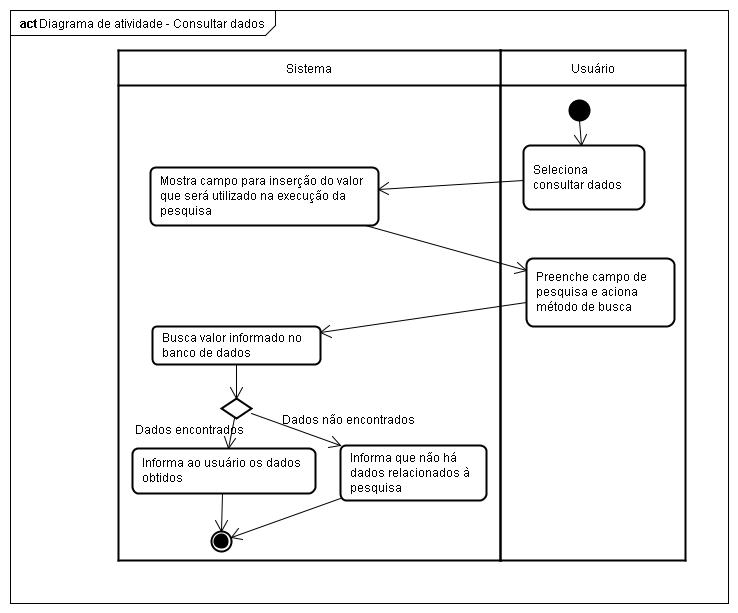
\includegraphics[width=15cm, height=20cm]{imagens-tc2/atividades/consultardados.jpg}
%\caption{Diagrama de atividade - Consultar dados}
\label{fig:Diagrama de atividade - Consultar dados}
\end{figure}
\begin{figure}
\centering
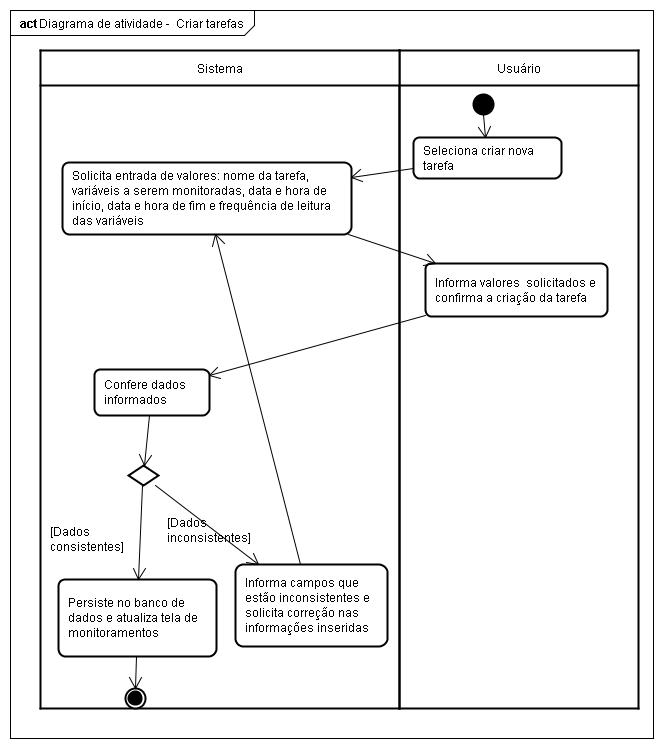
\includegraphics[width=15cm, height=20cm]{imagens-tc2/atividades/criartarefas.jpg}
%\caption{Diagrama de atividade - Criar tarefas}
\label{fig:Diagrama de atividade - Criar tarefas}
\end{figure}
\begin{figure}
\centering
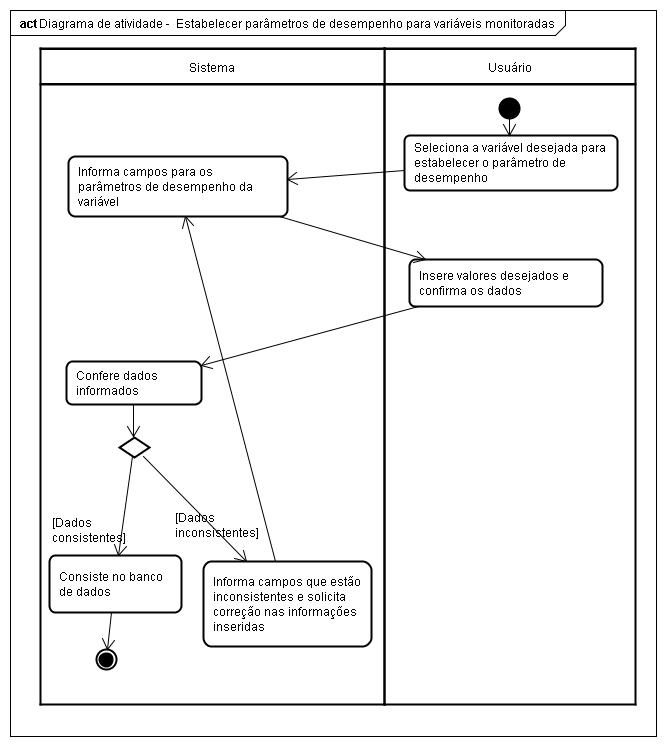
\includegraphics[width=15cm, height=20cm]{imagens-tc2/atividades/estabelecerparametros.jpg}
%\caption{Diagrama de atividade - Estabelecer par�metros de desempenho para vari�veis monitoradas}
\label{fig:Diagrama de atividade - Estabelecer par�metros de desempenho para vari�veis monitoradas}
\end{figure}
\begin{figure}
\centering
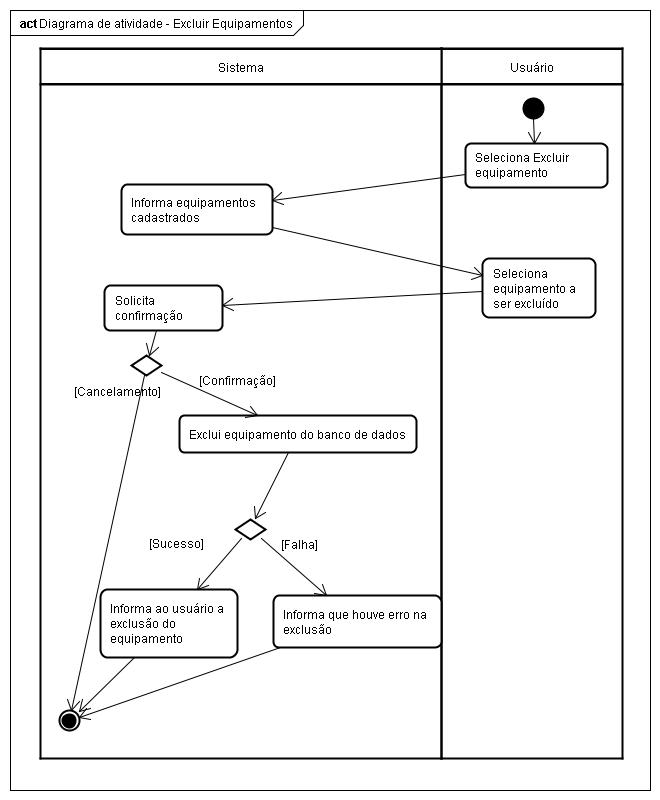
\includegraphics[width=15cm, height=20cm]{imagens-tc2/atividades/excluirequipamentos.jpg}
%\caption{Diagrama de atividade - Excluir Equipamentos}
\label{fig:Diagrama de atividade - Excluir Equipamentos}
\end{figure}
\begin{figure}
\centering
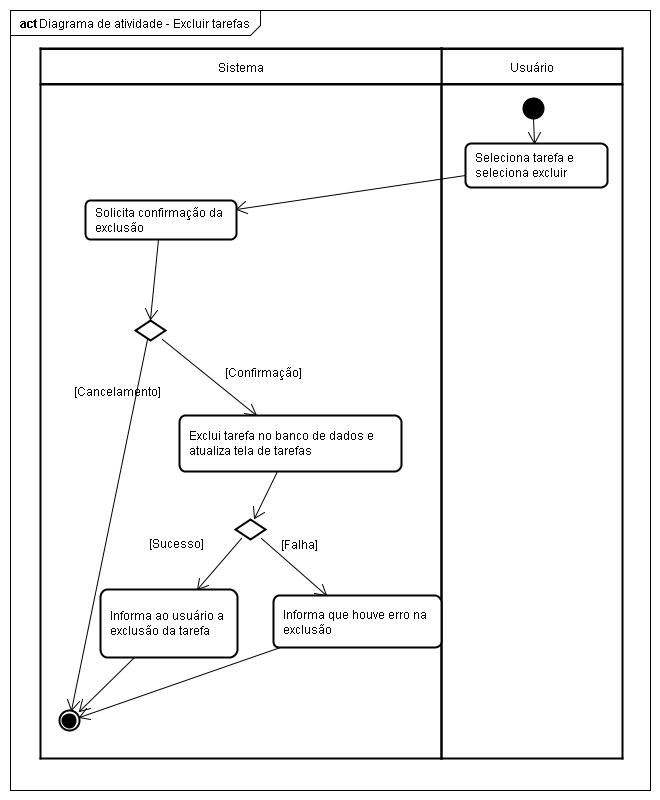
\includegraphics[width=15cm, height=20cm]{imagens-tc2/atividades/excluirtarefas.jpg}
%\caption{Diagrama de atividade - Excluir tarefas}
\label{fig:Diagrama de atividade - Excluir tarefas}
\end{figure}
\begin{figure}
\centering
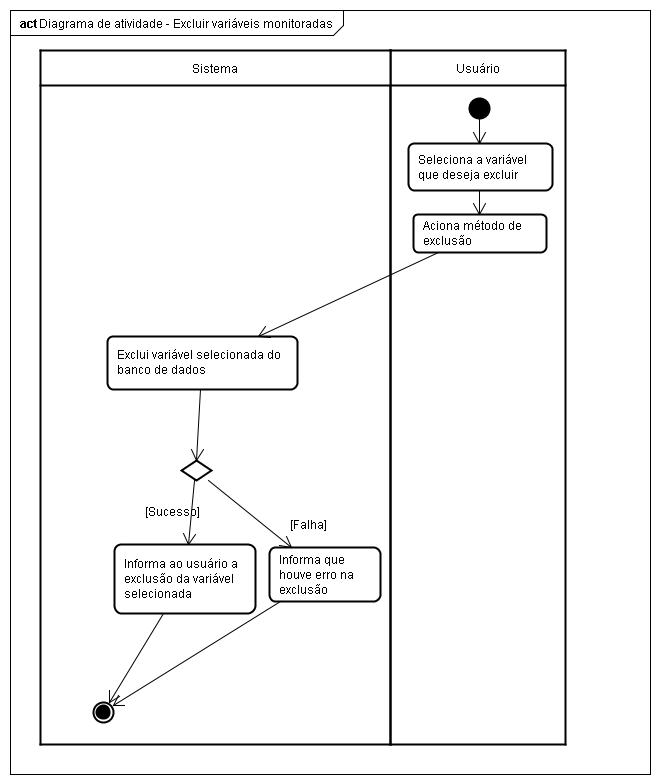
\includegraphics[width=15cm, height=20cm]{imagens-tc2/atividades/excluirvariaveis.jpg}
%\caption{Diagrama de atividade - Excluir vari�veis monitoradas}
\label{fig:Diagrama de atividade - Excluir vari�veis monitoradas}
\end{figure}
\begin{figure}
\centering
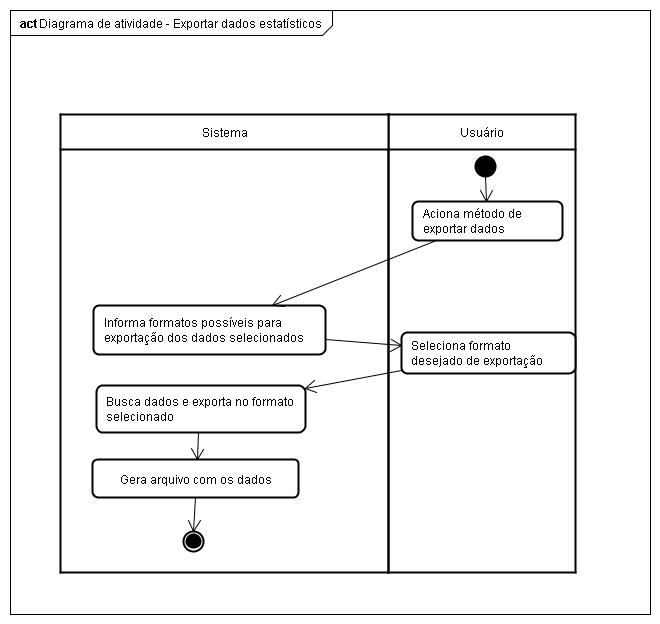
\includegraphics[width=15cm, height=20cm]{imagens-tc2/atividades/exportardados.jpg}
%\caption{Diagrama de atividade - Exportar dados estat�sticos}
\label{fig:Diagrama de atividade - Exportar dados estat�sticos}
\end{figure}
\begin{figure}
\centering
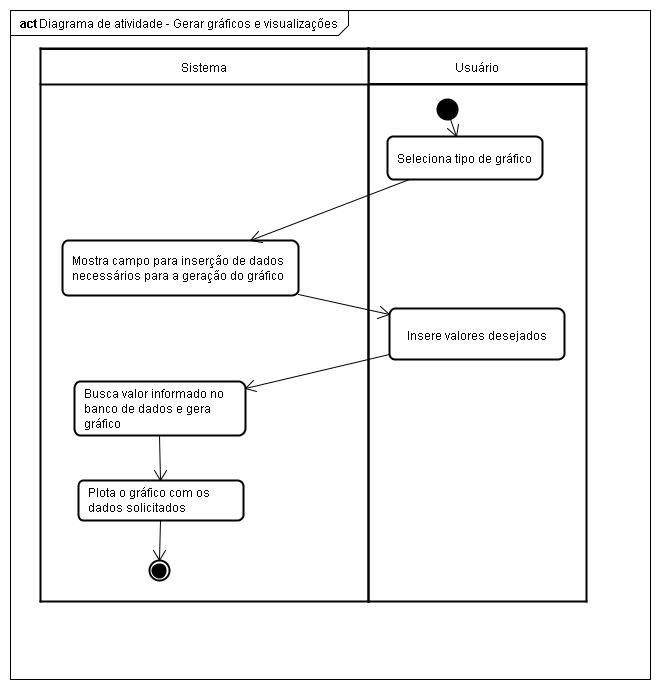
\includegraphics[width=15cm, height=20cm]{imagens-tc2/atividades/gerargraficos.jpg}
%\caption{Diagrama de atividade - Gerar gr�ficos e visualiza��es}
\label{fig:Diagrama de atividade - Gerar gr�ficos e visualiza��es}
\end{figure}
\begin{figure}
\centering
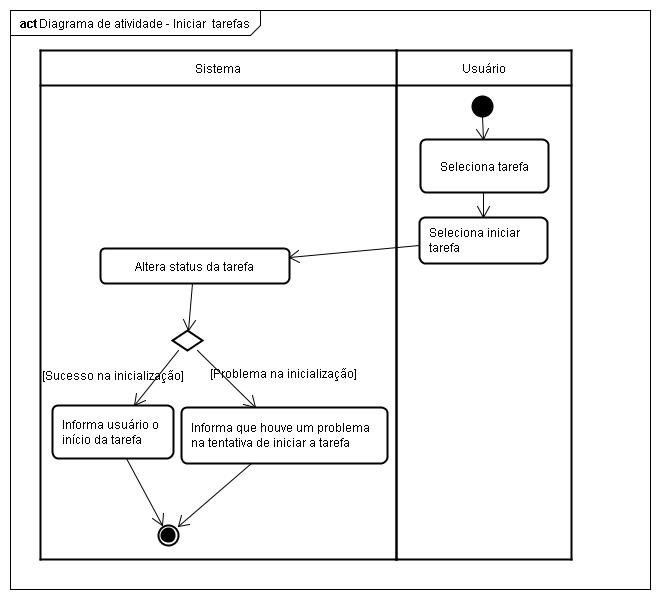
\includegraphics[width=15cm, height=20cm]{imagens-tc2/atividades/iniciartarefas.jpg}
%\caption{Diagrama de atividade - Iniciar tarefas}
\label{fig:Diagrama de atividade - Iniciar tarefas}
\end{figure}
\begin{figure}
\centering
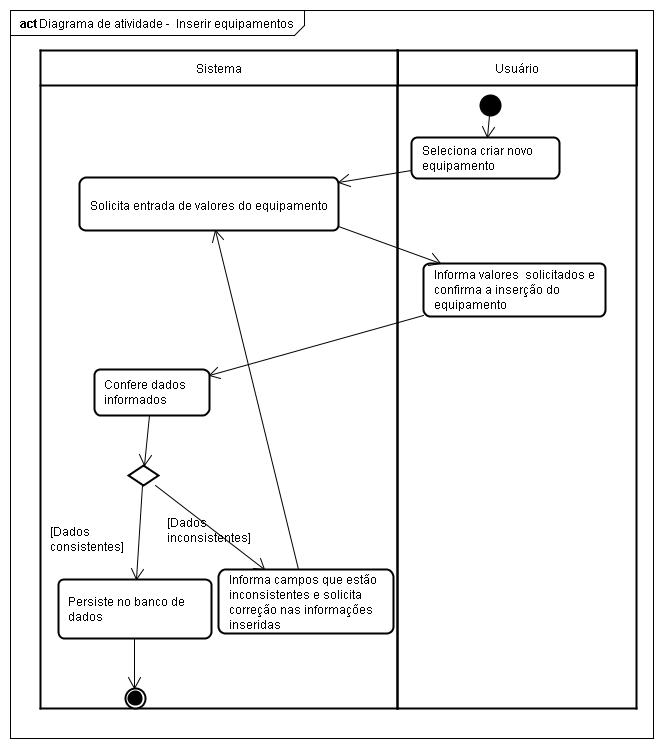
\includegraphics[width=15cm, height=20cm]{imagens-tc2/atividades/inserirequipamentos.jpg}
%\caption{Diagrama de atividade - Inserir equipamentos}
\label{fig:Diagrama de atividade - Inserir equipamentos}
\end{figure}
\begin{figure}
\centering
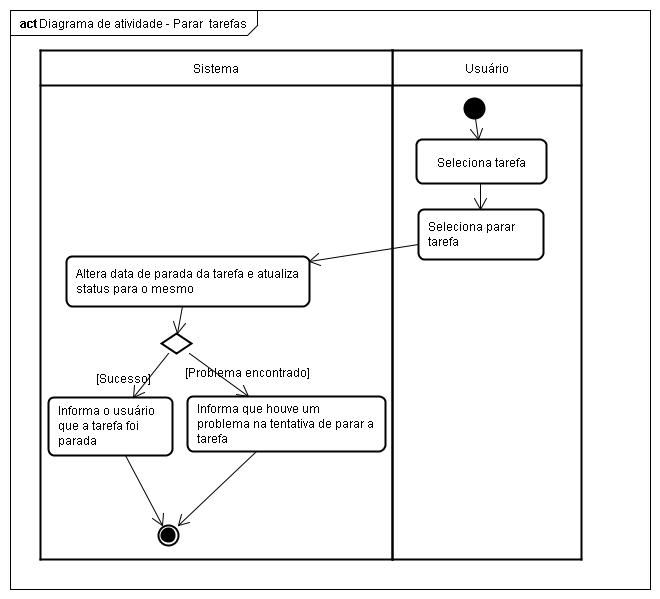
\includegraphics[width=15cm, height=20cm]{imagens-tc2/atividades/parartarefas.jpg}
%\caption{Diagrama de atividade - Parar tarefas}
\label{fig:Diagrama de atividade - Parar tarefas}
\end{figure}

\chapter*{Anexo B --- Diagramas de Classes}
\label{anexo}
%\addtocontents{toc}{\protect\contentsline {chapter}{Anexo B --- Diagramas de Classes}{74}}
Neste anexo s�o apresentados os diagramas de classes UML modelados para a implementa��o do sistema. S�o apresentados os diagrama de classes, inicialmente uma figura contendo todos os pacotes e classes (Figura \ref{classes:all}). A seguir cada um dos pacotes � melhor detalhado nas demais figuras.
\par O pacote \textit{model} cont�m as classes que s�o as entidades do programa, os DAOs de acesso �s entidades e enumera��es utilizadas nas classes entidades (Figura \ref{classes:model}).
\par O pacote \textit{controller} cont�m as classes de controle de acesso �s classes DAOs e classes de acesso ao protocolo SNMP (Figura \ref{classes:controller}).
\par O pacote \textit{util} cont�m as classes de utilidades do sistema, como configura��o de acesso ao banco de dados, exporta��o de dados, mensagens de erros do sistema, escalonador de leituras e classe inicial do sistema (Figura \ref{classes:util}).
\par Os pacotes \textit{graphics} e \textit{charts} cont�m as classes que geram as visualiza��es do sistema (Figura \ref{classes:graphics} e Figura \ref{classes:charts}).
\par E, o pacote \textit{view} cont�m as classes que representam as janelas e interfaces gr�ficas do sistema (Figura \ref{classes:view}).
\begin{figure}
\centering
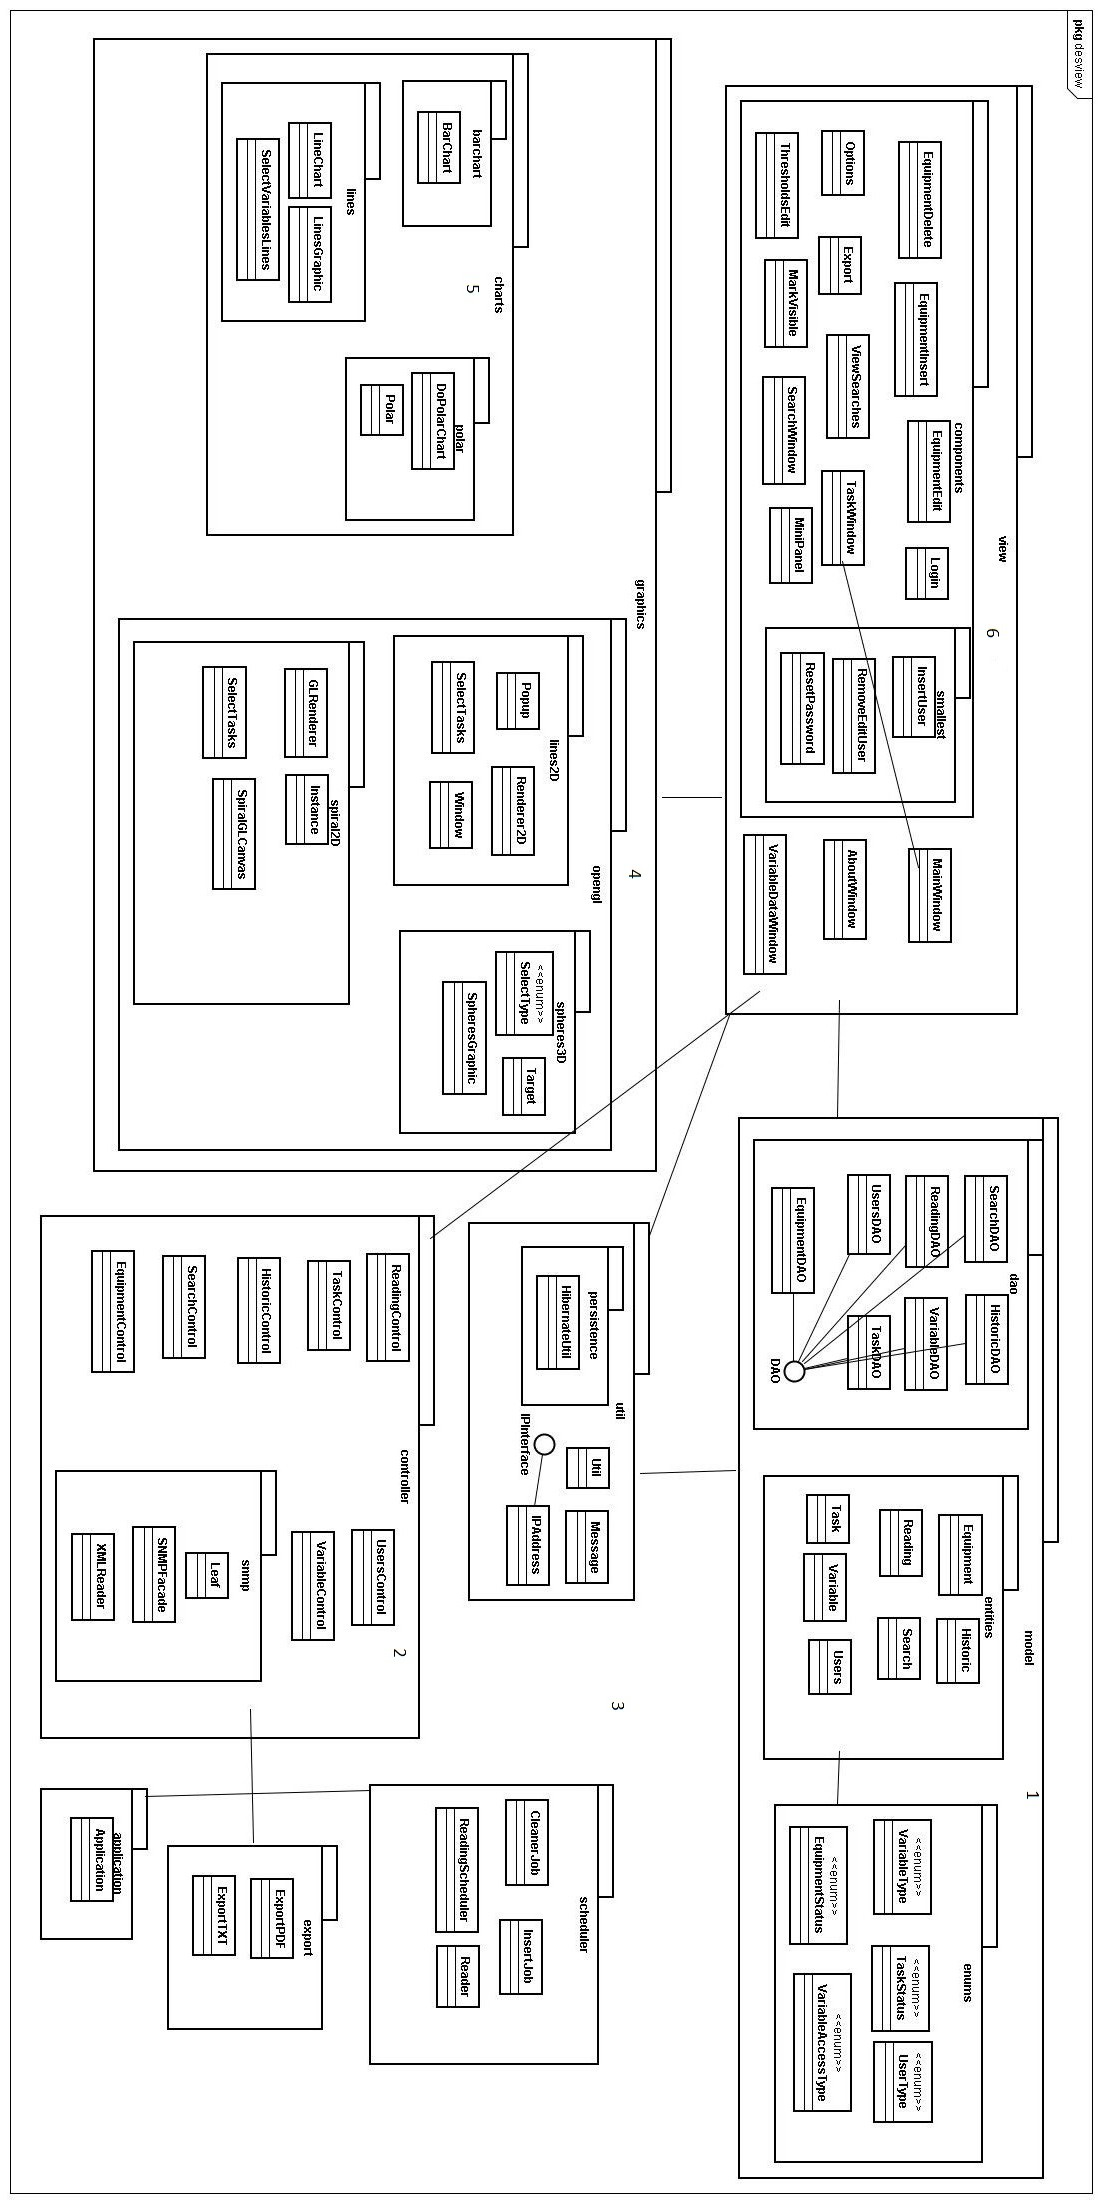
\includegraphics[width=16cm, height=20cm]{imagens-tc2/classes/allclasses.jpg}
\caption{Modelo conceitual de classes do sistema}
\label{classes:all}
\end{figure}
\begin{figure}
\centering
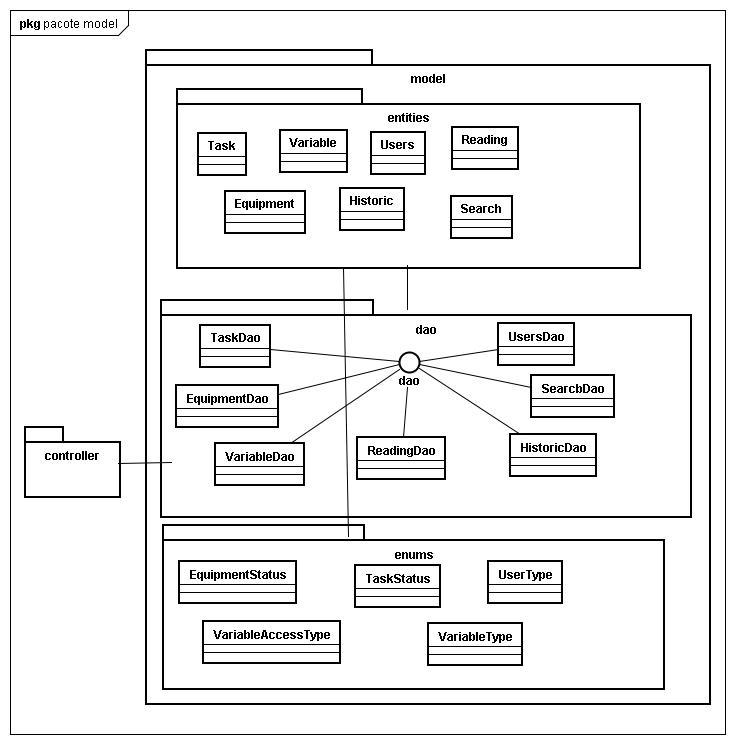
\includegraphics[width=15cm, height=20cm]{imagens-tc2/classes/model.jpg}
\caption{Modelo conceitual de classes: parte 1 - pacote \textit{model}.}
\label{classes:model}
\end{figure}
\begin{figure}
\centering
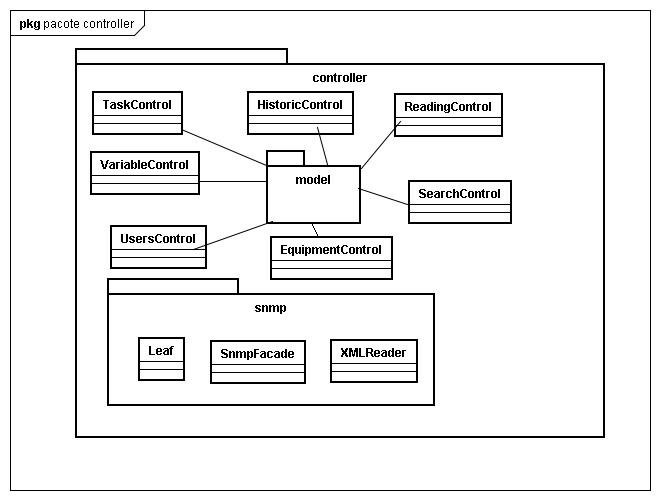
\includegraphics[width=15cm, height=20cm]{imagens-tc2/classes/controller.jpg}
\caption{Modelo conceitual de classes: parte 2 - pacote \textit{controller}.}
\label{classes:controller}
\end{figure}
\begin{figure}
\centering
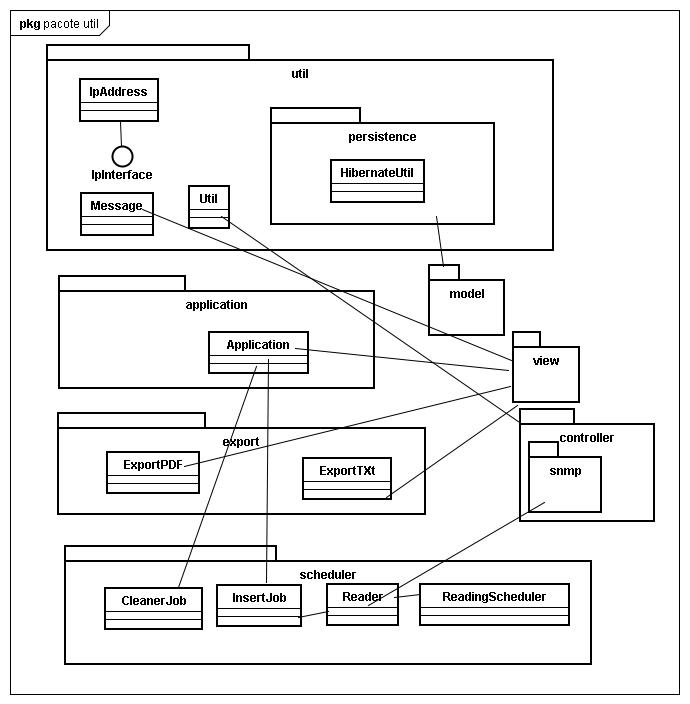
\includegraphics[width=15cm, height=20cm]{imagens-tc2/classes/util.jpg}
\caption{Modelo conceitual de classes: parte 3 - pacote \textit{util}.}
\label{classes:util}
\end{figure}
\begin{figure}
\centering
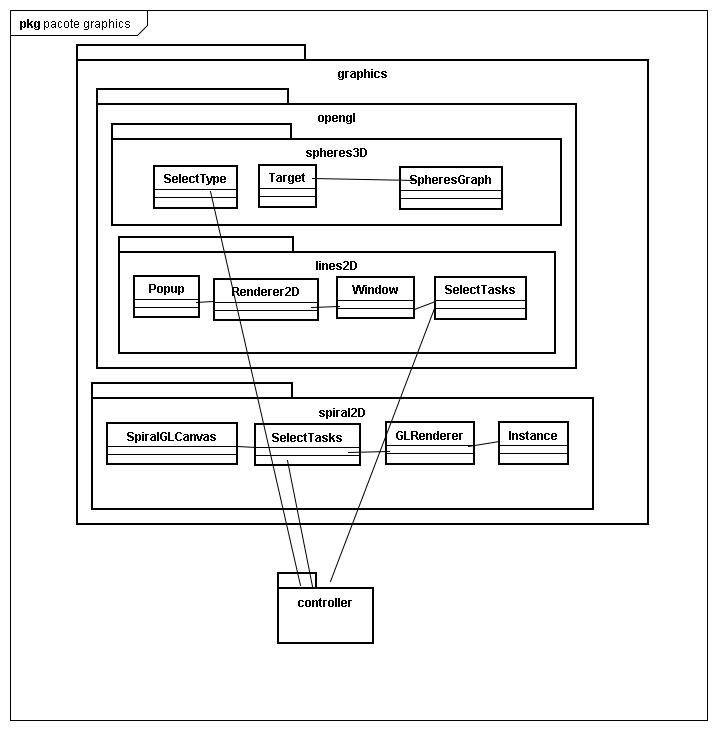
\includegraphics[width=15cm, height=20cm]{imagens-tc2/classes/graphics.jpg}
\caption{Modelo conceitual de classes: parte 4 - pacote \textit{graphics}.}
\label{classes:graphics}
\end{figure}
\begin{figure}
\centering
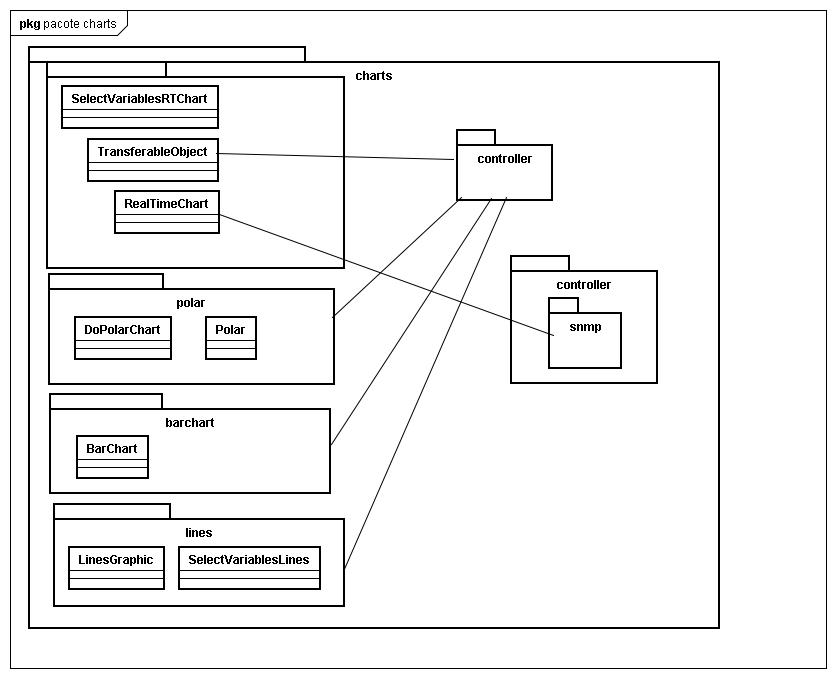
\includegraphics[width=15cm, height=20cm]{imagens-tc2/classes/charts.jpg}
\caption{Modelo conceitual de classes: parte 5 - pacote \textit{chart}s.}
\label{classes:charts}
\end{figure}
\begin{figure}
\centering
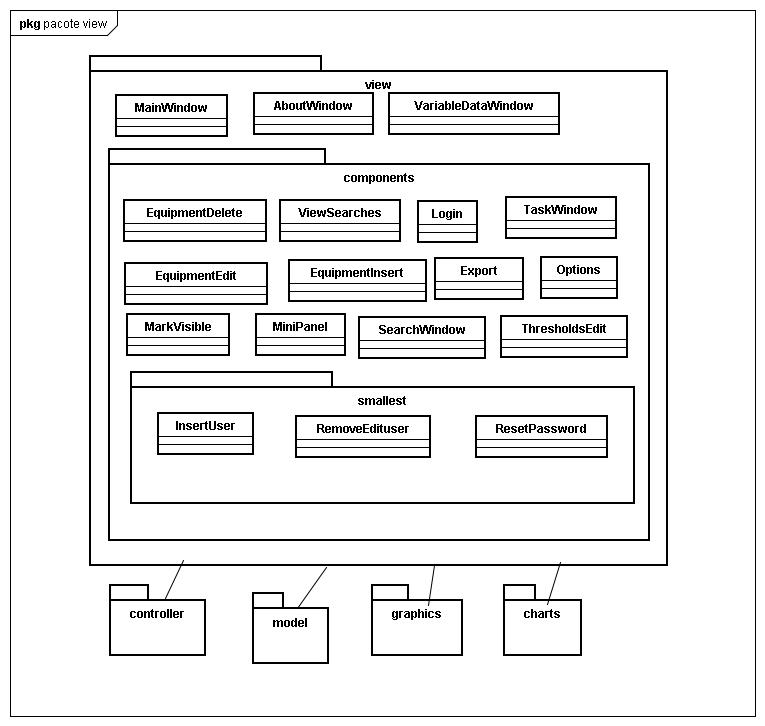
\includegraphics[width=15cm, height=20cm]{imagens-tc2/classes/view.jpg}
\caption{Modelo conceitual de classes: parte 6 - pacote \textit{view}.}
\label{classes:view}
\end{figure}
